% !TeX root = ../main.tex
% Add the above to each chapter to make compiling the PDF easier in some editors.

\chapter{Introduction}\label{chapter:introduction}

\section{Learning}
Learning is a process which involves obtaining new behaviors, skills, preferences, attitudes and understanding \cite{holt2012}. The capability to learn is a characteristic of animals, some machines and to a certain extent, of plants \cite{karban2015}. Learning can be accumulated through a single event such as being burned by a stove but often it happens through repeated experiences \cite{schacter2011}. \\
The remainder of this section explains different types of learning and draws parallels between learning types and machine learning sub fields:
\begin{itemize}
    \item Non-associative learning: It is a type of learning which occurs due to repeated exposure to a stimulus which results in a learned reaction to the stimulus \cite{fuentes2017}. Supervised learning for machines \cite{bishop2006} is like non-associative learning as in, it involves learning to output a label as a reaction to an input.
    \item Associative learning: A subject learns an association between two events \cite{plotnik2013}. Unsupervised learning for machines \cite{bishop2006} is similar to associative learning because it often involves a model, learning to group inputs together and assigning a label to every group. In practice, non-associative and associative learning are used together for resolution of problems. Semi-supervised learning for machines \cite{bishop2006}, involves using supervised and unsupervised learning for machines in parallel.
    \item Active learning: A subject controls its course of learning. It is significant for a learner to identify what it understands and what it does not understand. This knowledge can have a positive impact on the learning process \cite{scott2012}. Active learning for machines \cite{settles2009} is loosely based on active learning, as it involves the computer deciding what to learn.
    \item Transfer learning: The transfer of knowledge and understanding to find a solution for a new problem. The knowledge and understanding is gained through resolving other problems \cite{perkins1989}. Transfer learning for machines \cite{bishop2006} is a similar concept to transfer learning, as transfer learning for machines involves information gained from a dataset being applied to a different dataset.
\end{itemize}

\section{Machine Learning}
Machine learning is the process that enables computers to perform tasks without hard-coding the solution programmatically by learning from data provided to them \cite{alpaydin2020}. Computers can be explicitly programmed to perform simple tasks such as arithmetic operations. For advanced tasks however, it becomes progressively more difficult to program computers explicitly e.g., a rule-based program performs worse than a machine learning program for classification of EEG spikes \cite{ganglberger2017}. For advanced tasks, it becomes more feasible to let a computer learn the steps which it needs to perform for successfully completing the tasks \cite{samuel1959}. \\
Machine learning deploys various approaches which allow the computer to learn to perform advanced tasks by finding out a suitable algorithm on its own without programming all the individual steps. A subset of machine learning approaches depend upon help in the form of labeled data i.e., to label the data so that the computer can find better solutions to the tasks in light of the information added through the labels \cite{bishop2006}. Machine learning approaches can be categorized into four categories:
\begin{itemize}
  \setlength\itemsep{0em}
  \item Supervised learning: The computer is provided with data which contains images and their respective labels. The computer aims to learns a generalized mapping from the images to the respective labels.
  \item Unsupervised learning: The computer is provided images without specifying the labels. The computer is expected to learn the inherent structure of the data based on the images.
  \item Semi-supervised learning: The computer learns a mapping from the inputs to outputs with help from data with labels as well as the data without labels. Semi-supervised learning can be the other way around too, where the computer learns the inherent structure of data with the help of labeled images in addition to images without any labels.
  \item Reinforcement learning: The computer tries to fulfill a goal by performing different actions within the environment.
\end{itemize}

\section{Deep Learning}
Deep learning models are typically based on ANNs. Convolutional Neural Networks (CNNs) \cite{fukushima1982} are the most used ANNs for deep learning for image processing tasks such as image classification, image segmentation etc. In deep learning several hidden layers of ANNs are stacked together. \\
The connecting pathways between the ANNs are given weights which are adjusted as the training process continues. The weights of the connections are increased or decreased depending upon the value of the input signals. ANNs are typically organized into layers. The output of each preceding layer is added as an input of the next layer. Each layer manipulates the input in a different way. The output of the last layer is used as the final prediction. \\
Deep learning involves several hidden layers stacked together in an ANN. Applications of deep learning include computer vision and natural language processing. \\
Each layer learns a different transformation of the inputs, which tend to be more abstract as the network gets deeper. For example, in case of an image of a car, in order to detect the image as a car, the first layer may learn the structure of pixels and the edges, the second layer may learn the arrangement of edges, the third layer may learn specific areas of the image such as wheels or steering, the fourth layer may learn the overall shape of the car. The main allure of deep learning models is that, the model can learn to place the features in different layers without any help. "Deep" refers to the number of layers of ANNs in a deep learning model \cite{bengio2013}. \\
Deep learning methods are typically optimized using stochastic gradient descent (SGD) \cite{bottou2010}. SGD requires a huge amount of data for training \cite{sun2017}.

\section{Active Learning}
Active learning \cite{settles2009} tries to mitigate the cost of labeling the datasets, by efficiently selecting the images, which can be labeled for maximum performance gain on the underlying task. \\
Active learning is a subfield of machine learning. The main idea behind active learning is that, the active learning algorithm chooses the images that the model should learn from. This is an important characteristic, because deep learning models can require thousands of labeled images to achieve good performance. More labeled data results in superior performance. Sometimes, the cost of obtaining labels is not high, e.g., the data obtained from users on social media or the data gathered by websites in a passive way about user behaviour but obtaining labels can be very costly and time-consuming. The cost of labels varies depending upon the complexity of the task. The cost of labels gets even higher in the biomedical domain. Due to the safety critical nature of medical data, multiple experts must be consulted for labeling biomedical datasets. \\
Hence, active learning algorithms try to achieve good performance while using as less images as possible. They do so, by selecting the images as shown in figure \ref{fig:active_learning}, which can have the most positive effect on the model's performance. As a result, active learning algorithms reduce the overall cost of labels.

\begin{figure}[htbp]
\centering
\captionsetup{format=plain}
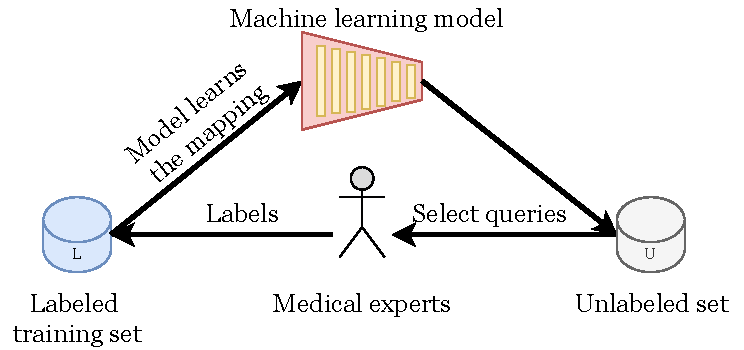
\includegraphics[width=0.75\textwidth]{figures/fig_active_learning.pdf}
\caption[Workflow of active learning]{\textbf{Workflow of active learning}. The labeled set $\mathcal{L}$ is used to train the model. The trained model is then used to select images, through an active learning algorithm, from the unlabeled set $\mathcal{U}$ for labeling. The selected images are labeled by an expert and added to the labeled set $\mathcal{L}$.}
\label{fig:active_learning}
\end{figure}

% make this bigger and take help from https://link.springer.com/article/10.1007/s10994-019-05855-6
\section{Semi-supervised Learning}
Semi-supervised learning (SSL) \cite{van2020} mitigates the requirement for labeled data by providing a means of leveraging unlabeled data. \\ Semi-supervised learning is a subfield of machine learning which tries to combine supervised learning with unsupervised learning. Semi-supervised learning algorithms try to use the information available in the unlabeled data domain to help the performance of the model in the labeled data domain or vice versa. For instance, in case of a classification task, the images without a label can help with the classification task. For an unsupervised method such as clustering, it can be helpful to have some images which are known to belong to a specific class. \\
There are many cases where unlabelled data can help in constructing a classifier. Consider the example of a regression model, where the model takes images of a house as input and it has to predict the price of a house. Suppose the model learns to predict a higher price for houses with a parking space compared to the houses which do not have this predictive property. This regression model might work well for the images in the training set that contain the predictive property of having a parking space but will fail when the input images do not contain that predictive property. For example, if a house does not have a parking space but it has other amenities such as a swimming pool, the model will still predict a lower price for that house. Semi-supervised learning can be helpful in this regard. Consider that the unlabeled dataset, might contain some images which connect the predictive property of having a parking space to the property of containing a swimming pool. For instance, the property of having a parking space might co-occur with the property of having a balcony. Moreover, the property of having a balcony might co-occur with the property of having a swimming pool. Hence, the model might be able to predict a higher price for a house containing a swimming pool, even if it has not seen that property in the training set.\\
SSL operates on the assumption that the unlabeled data contains some prior information about the labeled data. Since unlabeled data can often be obtained with minimal human labor, any performance boost conferred by SSL often comes with lower cost. \\

\begin{figure}[htbp]
\centering
\captionsetup{format=plain}
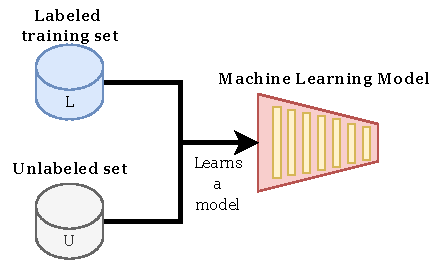
\includegraphics[width=0.65\textwidth]{figures/fig_semi_supervised_learning.pdf}
\caption[Workflow of semi-supervised Learning]{\textbf{Workflow of Semi-supervised Learning}. In semi-supervised learning (SSL), both, the labeled set $\mathcal{L}$ and the unlabeled set $\mathcal{U}$, are used for learning a model. The information in the unlabeled set $\mathcal{U}$ is harnessed to improve the training performance on labeled set $\mathcal{L}$.}
\label{fig:semi_supervised_learning}
\end{figure}

\section{Transfer Learning}
Transfer learning (TL) is a subfield of machine learning which focuses on applying the knowledge gained through resolving one problem, to another preferably similar problem \cite{west2007}. For example, knowledge gained through learning how to recognize bicycles can be applied to recognizing motor bikes. From a practical point of view, reusing and transferring of information gained through one task to another can result in label-efficient learning e.g., it is possible that one has access to a large labeled dataset which contains thousands of images, however the dataset that the learning has to carried out on, is small with relatively few labels. Through TL, it is possible to learn a model on the large dataset and then use the learned model weights for achieving better performance on the smaller dataset \cite{pan2009}. 

\section{Self-supervised Learning}
Self-supervised learning's basic idea is to automatically create a supervistory signal to solve a task \cite{nava2019}. In terms of computer vision, self-supervised learning is applied to representation learning. Here, a model is learnt by a self-supervised strategy i.e., by generating a automatic supervision signal and then the learned model is used for further training on labeled data. Self-supervised learning is useful, when the labeled data is scarce while there is a large amount of unlabeled data available.  \\
In self-supervised learning for representation learning, the features are learned using pretext tasks. Pretext tasks can include, predict the rotation of an augmented image \cite{gidaris2018} or to recognize augmented versions of an image \cite{chen2020} etc.

\section{Label-efficient Deep Learning}
Deep learning methods are dependent upon large amounts of labeled data for their success \cite{sun2017}. In case of biomedical images, the labeling must be carried out by trained experts, so the process of labeling is time-consuming and expensive. Active learning algorithms try to minimize the need of labels by selecting the images which are most informative for labeling \cite{settles2009, sadafi2019, joshi2009}, but these algorithms are usually tested on real world image datasets e.g., ImageNet \cite{gal2016, ducoffe2015, holub2008}. However, biomedical images do not posses the same properties as real world images. Biomedical images have little variation between classes and posses little difference in color and textures \cite{matek2019, esteva2017}. Furthermore, biomedical image datasets typically have high class imbalance, which can have a significant impact on the results e.g., an algorithm which performs quite good for a dataset with no class imbalance might not perform as well for a dataset with high class imbalance. It has been shown that active learning can work well for biomedical image classification \cite{sadafi2019, smailagic2018} and segmentation \cite{yang2017}. However, it is not clear that which active learning algorithm is more suited for a particular kind of biomedical image data and how can the active learning algorithms be combined with other deep learning methods for improving their performance. \\
It has been shown that pre-training methods such as transfer learning and self-supervised pre-training show great promise for initialization of network weights when low amount of labeled data is available \cite{chen2020, oord2018, newell2020, sagheer2019}. For transfer learning, the network weights are learned by training on a different dataset (preferably similar) and then reusing the learned weights for network initialization while training on the target dataset \cite{jing2020}. Initialization using pre-trained ImageNet weights is the most common transfer learning method and has been used in many biomedical applications for network initialization \cite{rajpurkar2017, wang2017}. However, it is shown by Raghu and Zhang et al. \cite{raghu2019} that in transfer learning using ImageNet weights might not lead to an improvement in the performance for many biomedical image datasets. Moreover, it is shown that self-supervised learning on biomedical images can lead to an increase in performance \cite{holmberg2020}. \\
Finally, semi-supervised learning has been shown to increase the performance and stability of results \cite{sohn2020, tarvainen2017}. High-throughput methods are regularly employed in biomedical imaging \cite{blasi2016} to obtain a large number of unlabeled images. However, as mentioned earlier, labels are scarce in the domain of biomedical imaging. Thus, semi-supervised methods have great potential in this domain. \\

\section{Research Goals}
In this thesis, firstly, a comparison has been made between different active learning methods. Secondly, the performance of the active learning algorithm which performed the best, is further improved by adding pre-training and semi-supervised learning. To find out if a certain combination of the three active learning algorithms in addition to random sampling (baseline), three pre-training methods plus random initialization (baseline) and two training strategies which include supervised and semi-supervised learning, can outperform other conventional methods, an extensive grid search is performed, and the results are gathered on three biomedical image datasets. As a result, an optimal strategy is found. In the following chapters, the biomedical datasets to be tested in this thesis are detailed in chapter \ref{chapter:datasets}. The active learning algorithms, pre-training methods and training strategies used in this thesis are detailed in chapter \ref{chapter:methods}. In chapter \ref{chapter:experiments}, implementation details and details about the hyper-parameters are provided. The results of all the testing on the biomedical datasets from chapter \ref{chapter:datasets} using the methods from chapter \ref{chapter:methods}, are shown in chapter \ref{chapter:results}. Lastly, a conclusion of the thesis is provided in chapter \ref{chapter:conclusion}.